%%%%%%%%%%%%%%%%%%%%%%%%%%%%%%%%%%%%%%%%%
% Beamer Presentation
% LaTeX Template
% Version 1.0 (10/11/12)
%
% This template has been downloaded from:
% http://www.LaTeXTemplates.com
%
% License:
% CC BY-NC-SA 3.0 (http://creativecommons.org/licenses/by-nc-sa/3.0/)
%
%%%%%%%%%%%%%%%%%%%%%%%%%%%%%%%%%%%%%%%%%

%----------------------------------------------------------------------------------------
%	PACKAGES AND THEMES
%----------------------------------------------------------------------------------------

\documentclass[russian,english,hyperref=unicode]{beamer}
\usepackage{cmap}
\usepackage[utf8]{inputenc}
\usepackage[T2A]{fontenc}
\usepackage[russian,english]{babel}
\usepackage{mathptmx}
\selectlanguage{russian}
\mode<presentation> {

% The Beamer class comes with a number of default slide themes
% which change the colors and layouts of slides. Below this is a list
% of all the themes, uncomment each in turn to see what they look like.

%\usetheme{default}
%\usetheme{AnnArbor}
%\usetheme{Antibes}
%\usetheme{Bergen}
%\usetheme{Berkeley}
%\usetheme{Berlin}
%\usetheme{Boadilla}
%\usetheme{CambridgeUS}
%\usetheme{Copenhagen}
%\usetheme{Darmstadt}
%\usetheme{Dresden}
%\usetheme{Frankfurt}
%\usetheme{Goettingen}
%\usetheme{Hannover}
%\usetheme{Ilmenau}
%\usetheme{JuanLesPins}
%\usetheme{Luebeck}
\usetheme{Madrid}
%\usetheme{Malmoe}
%\usetheme{Marburg}
%\usetheme{Montpellier}
%\usetheme{PaloAlto}
%\usetheme{Pittsburgh}
%\usetheme{Rochester}
%\usetheme{Singapore}
%\usetheme{Szeged}
%\usetheme{Warsaw}

% As well as themes, the Beamer class has a number of color themes
% for any slide theme. Uncomment each of these in turn to see how it
% changes the colors of your current slide theme.

%\usecolortheme{albatross}
%\usecolortheme{beaver}
%\usecolortheme{beetle}
%\usecolortheme{crane}
%\usecolortheme{dolphin}
%\usecolortheme{dove}
%\usecolortheme{fly}
%\usecolortheme{lily}
%\usecolortheme{orchid}
%\usecolortheme{rose}
%\usecolortheme{seagull}
%\usecolortheme{seahorse}
%\usecolortheme{whale}
%\usecolortheme{wolverine}

%\setbeamertemplate{footline} % To remove the footer line in all slides uncomment this line
%\setbeamertemplate{footline}[page number] % To replace the footer line in all slides with a simple slide count uncomment this line
\setbeamertemplate{footline}{\hfill\insertframenumber/\inserttotalframenumber} 

\setbeamertemplate{navigation symbols}{} % To remove the navigation symbols from the bottom of all slides uncomment this line

\setbeamercovered{transparent}
\usenavigationsymbolstemplate{}

}
\usepackage{graphicx} % Allows including images
\usepackage{booktabs} % Allows the use of \toprule, \midrule and \bottomrule in tables
%\usepackage {tikz}
\usepackage{tkz-graph}
\GraphInit[vstyle = Shade]
\tikzset{
  LabelStyle/.style = { rectangle, rounded corners, draw,
                        minimum width = 2em, fill = yellow!50,
                        text = red, font = \bfseries },
  VertexStyle/.append style = { inner sep=5pt,
                                font = \normalsize\bfseries},
  EdgeStyle/.append style = {->, bend left} }
\usetikzlibrary {positioning}
%\usepackage {xcolor}
\definecolor {processblue}{cmyk}{0.96,0,0,0}
%----------------------------------------------------------------------------------------
%	TITLE PAGE
%----------------------------------------------------------------------------------------

\title[Short title]{Построение представления группы по машине Тьюринга} % The short title appears at the bottom of every slide, the full title is only on the title page

\author{Шамрай Максим} % Your name
\institute[Лаборатория языковых инструментов] % Your institution as it will appear on the bottom of every slide, may be shorthand to save space
{
Лаборатория языковых инструментов\\ % Your institution for the title page
\medskip
}
\date{14.12.2019} % Date, can be changed to a custom date

\begin{document}
\selectlanguage{russian}
\begin{frame}
\titlepage % Print the title page as the first slide
\end{frame}

%\begin{frame}
%\frametitle{Overview} % Table of contents slide, comment this block out to remove it
%\tableofcontents % Throughout your presentation, if you choose to use \section{} and \subsection{} %commands, these will automatically be printed on this slide as an overview of your presentation
%\end{frame}

%----------------------------------------------------------------------------------------
%	PRESENTATION SLIDES
%----------------------------------------------------------------------------------------

%------------------------------------------------

\begin{frame}\frametitle{Мотивация}

\begin{center}
    $R \subset CF \subset Conj \subseteq Bool$
\end{center}
\begin{itemize}
    \item Кроме всем известной иерархии Хомского, есть довольно много классов формальных языков
    \item И не все они имеют свою лемму о накачке
    \item В последнее время все чаще прибегают к смежным дисциплинам для исследования языков
    \item Мы предлагаем построить группу по языку, чтобы в дальнейшем можно было применять аппарат теории групп для исследований
\end{itemize}

\end{frame}

%%%%%%%%%%%%%%%%%%%%%%%%%%%%%%%%%%%%%%%%%%%%%%%%%%%%%%%%%%%%%%%%%%%%%%%%%%%%%%%
%%%%%%%%%%%%%%%%%%%%%%%%%%%%%%%%%%%%%%%%%%%%%%%%%%%%%%%%%%%%%%%%%%%%%%%%%%%%%%%

\begin{frame}{Связь с теорией групп}
    \begin{center}
        Пусть $\Sigma$ --- конечный алфавит, тогда
    \end{center}
    \begin{itemize}
        \item $\Sigma^+$ --- свободная полугруппа
        \item $\Sigma^*$ --- свободный моноид
        \item $(\Sigma \cup \Sigma^{-1})^*$ --- свободная группа
    \end{itemize}
    \pause
    \begin{center}
        $G = \langle A~|~R \rangle$ --- представление группы, 
        где $A$ --- множество образующих, $R$ --- множество определяющих отношений
    \end{center}
    \begin{itemize}
        \item $G = \langle a, b~|~a^3, b^2, (ab)^2 \rangle = \{\epsilon, a, a^2, b, ab, a^2b\} = Sym_3$
        \item $G = \langle a~|~a^5\rangle = C_5$
        \item $G = \langle a, b~|~aba^{-1}b^{-1} \rangle$
    \end{itemize}
    \pause
    \begin{block}{Теорема 1}
		Пусть $L \subseteq \Sigma^+$ язык, принимаемый машиной Тьюринга $M$,
    тогда существует конечно заданная группа $G(M)=\langle A~|~R \rangle$
    и инъективное отображение $K: \Sigma^+ \to (A \cup A^{-1})^+$ такое что:
    $u \in L \iff K(u)=1_G$
	\end{block}
\end{frame}

\begin{frame}{Цели}
    \begin{enumerate}
        \item Реализовать алгоритм построения группы по машине Тьюринга, основываясь на доказательстве предыдущей теоремы
        \item Доказать корректность алгоритма
    \end{enumerate}
\end{frame}

\begin{frame}{Построение группы (0)}
\begin{block}{Теорема 2}
Для любой машины Тьюринга M существует симметричная машина Тьюринга M' со следующими свойствами:
    \begin{itemize}
        \item Распознает тот же язык, что и M
        \item Каждая команда действует только на одной ленте
        \item Добавляется лента, алфавитом которой являются команды
    \end{itemize}
\end{block}
\pause
\begin{block}{Теорема 3}
Для любой машины Тьюринга M', удовлетворяющей теореме 2, существует S-машина, которая симулирует M'
\end{block}
\pause
\begin{block}{Теорема 4}
Для любой S-машины, удовлетворяющей теореме 3, существует соответствующая конечно представленная группа
\end{block}
\end{frame}

\begin{frame}{Построение группы (1)}
\begin{figure}[H]
  \centering
  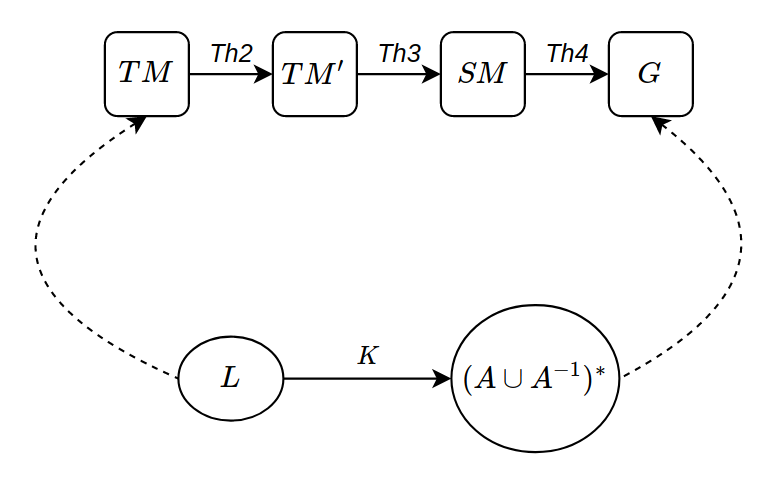
\includegraphics[width=120mm]{1.png}
 \end{figure}
\end{frame}

\begin{frame}{Результаты и дальнейшие действия}
    \begin{itemize}
        \item На данный момент алгоритм уже реализован
        \item Был проведен ряд экспериментов
        \item Найдена более свежая статья, где присутствуют похожие преобразования
        \item Рассматривается возможность формальной верификации алгоритма
    \end{itemize}
\end{frame}

\end{document}